\begin{defproblem}{install}
  \begin{onlyproblem}
    Install Scratch on your machine.
  \end{onlyproblem}
\end{defproblem}

\begin{defproblem}{helloWorld}
  \begin{onlyproblem}
    Make your own ``hello world'' Scratch-program. The program must make
    default sprite say ``Hello World'' when you press the green flag.
  \end{onlyproblem}
\end{defproblem}

\begin{defproblem}{moveIt}
  \begin{onlyproblem}
    Make a Scratch program with a sprite of your own choosing, which
    moves on the screen using the 'glide' and the 'forever' loop.
  \end{onlyproblem}
\end{defproblem}

\begin{defproblem}{screenShots}
  \begin{onlyproblem}
    Take one or more screenshots of one of your Scratch-programs while it runs.
  \end{onlyproblem}
\end{defproblem}

\begin{defproblem}{countDown}
  \begin{onlyproblem}
    Make a Scratch-program, which counts down from 10 to 1. You must use a
    variable and a repeat loop.
  \end{onlyproblem}
\end{defproblem}

\begin{defproblem}{countDownWhenPressed}
  \begin{onlyproblem}
    Make a Scratch-program, which counts down from 10 to 1. The countdown must
    first start, when you press the mouse.
  \end{onlyproblem}
\end{defproblem}

\begin{defproblem}{countDoubles}
  \begin{onlyproblem}
    Make a Scratch-program, which counts up every even number from 0 to 20.
  \end{onlyproblem}
\end{defproblem}

\begin{defproblem}{game}
  \begin{onlyproblem}%
    Design a game in Scratch:\\
    You are to design a game of your own choosing. The game must
    \begin{itemize}
    \item include 2--5 sprites 
    \item have a typical gameplay of about 1 minute
    \item must include at least 1 variable
    \end{itemize}
    You may use any existing block in Scratch, and the game may be
    similar to an existing game. The graphical appeal and the sound
    aspects of the games is of littel importance.

    A good approach is to:
    \begin{enumerate}
    \item Start by brainstorming about a game, you would like to make
      and what the game mechanics should be.
    \item Make a design on paper about the gameplay.
    \item Implement your design as a sketch of a Scratch program, still on paper.
    \item Enter your prototype into Scratch and test it.
    \item Return to the top and update your game until you are satisfied with the result.
    \end{enumerate}
  \end{onlyproblem}
\end{defproblem}

\begin{defproblem}{10Blocks}
  \begin{onlyproblem}%
    What can you make with 10 Scratch-blocks?\\
    In Figur~\ref{fig:blokke} is shown 10 Scratch-blocks.
    \begin{figure}
      \centering
      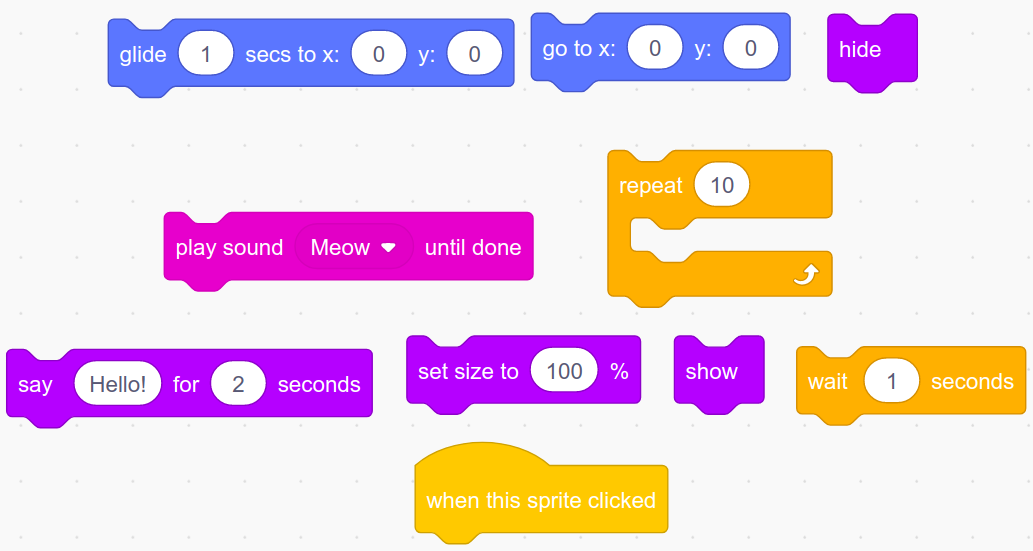
\includegraphics[width=0.9\linewidth]{figures/Scratch3.png}
      \caption{10 Scratch-blokke}
      \label{fig:blokke}
    \end{figure}
    Your task is to make a fun program only by using these blocks. Each block may be used 0 or mor times. Try to connect the blocks first on paper, write what you think, it will do and then enter the program in Scratch and run it. Describe to what extent the program did as expected.
  \end{onlyproblem}
\end{defproblem}

%%%%%%%%%%%%%%%%%%%%%%%%%%%

\begin{defproblem}{commandLine}
  \begin{onlyproblem}[fragile]
    Start the command line (or terminal on MacOS), select and use \texttt{cd} to move the filepointer to a suitable place for your work. Create a directory from the command line. Use a text-editor to create a \LaTeX\ document using the class \texttt{article}. The preamble must define the title ``Hello world'', your name as the author, and today's date as the date. The main part of the document must use \verb\maketitle ~to produce the title and the text ``Hello again''. Convert the \LaTeX\ to \texttt{pdf} from the command line.
  \end{onlyproblem}
\end{defproblem}

\begin{defproblem}{report}
  \begin{onlyproblem}[fragile]%
    Write a short report in \LaTeX\ with Emacs and translate the
    \lstinline[language=console]{tex}-file to a
    \lstinline[language=console]{pdf}-file using the command line. The
    report should as minimum contain:
     \begin{itemize}
     \item A title produced using \verb\maketitle, 
     \item A section with a section title using \verb\section,
     \item One or more figures of screenshots from your program and
       by using the \verb figure ~environment, and it
       must include a caption text using \verb\caption.
     \item A reference to the figure using the \verb\label--\verb\ref\ pair.
     \item The Danish letters 'æ', 'ø', and 'å'.
    \end{itemize}
  \end{onlyproblem}
\end{defproblem}

%%%%%%%%%%%%%%%%%%%%%%%%%%%

\begin{defproblem}{add}
  \begin{onlyproblem}%
    \label{ex:interactiveSession}
    Start an interactive F\# session and type the following ending with a newline: \lstinline{3.14+2.78;;} Describe what F\# did and if there was an error, find it and repeat.
  \end{onlyproblem}
\end{defproblem}

\begin{defproblem}{compile}
  \begin{onlyproblem}%
    Repeat Exercise~\ref{ex:interactiveSession}, but this time, type the code in a text editor and save the result in a file with the suffix \texttt{.fsx}. Run through \lstinline[language=console]{fsharpi} from the console, and by first compiling it with \lstinline[language=console]{fsharpc} and executing the compiled file using \lstinline[language=console]{mono}. Consider whether the result was as expected and why.
  \end{onlyproblem}
\end{defproblem}

\begin{defproblem}{interpretVsCompile}
  \begin{onlyproblem}%
    Describe the 3 ways, an F\# program can be run from the command line (terminal), and discuss the advantages and disadvantages of each method.s.
  \end{onlyproblem}
\end{defproblem}

\begin{defproblem}{concat}
  \begin{onlyproblem}%
    Write an expression which concatenates the strings \lstinline{"hello"}, \lstinline{" "}, \lstinline{"world"} and run it in F\#.
  \end{onlyproblem}
\end{defproblem}

\begin{defproblem}{typeError}
  \begin{onlyproblem}%
    Type the following expression in F\# interactive mode, \lstinline{3 + 1.0;;} and explain the result. Consider whether you can improve the expression.
  \end{onlyproblem}
\end{defproblem}

\begin{defproblem}{divideBy2ByHand}
  \begin{onlyproblem}%
    Using pen and paper:
    \begin{textenum}
    \item Write the integer $3_{10}$ on binary form by using the divide-by-2 algorithm.
    \item Write the integer $1001_2$ on decimal form using the multiply-by-2 algorithm.
    \item Write the integer $47_{10}$ on hexadecimal and octal form.
    \end{textenum}
  \end{onlyproblem}
\end{defproblem}

\begin{defproblem}{otherBases}
  \begin{onlyproblem}%
    Enter the integer $47_{10}$ on decimal, hexadecimal, octal, og floating-point form in F\# and verify that all represents the same value.
\end{onlyproblem}
\end{defproblem}

\begin{defproblem}{truthTable}
  \begin{onlyproblem}%
    Write the truth table for the boolean expression $a \text{ \texttt{\bf or} } b \text{ \texttt{\bf and} } c$, where $a$, $b$, and $c$ are boolean values.
  \end{onlyproblem}
\end{defproblem}

\begin{defproblem}{uy}
  \begin{onlyproblem}%
    Consider the F\#-expression \lstinline{164uy+230uy}. Explain what \lstinline{"uy"} means, compute the expression with \lstinline[language=console]{fsharpi}, and discuss the result.
  \end{onlyproblem}
\end{defproblem}

\begin{defproblem}{unicode}
  \begin{onlyproblem}%
    Write an F\#-expression for a string that contains the characters ``edb'' solely by using unicode escape codes.
  \end{onlyproblem}
\end{defproblem}

\begin{defproblem}{slicing}
  \begin{onlyproblem}%
    Write an F\#-expression which extracts the 3.\ element and the substring from the 2.\ to the 4.\ element in the string ``abcdef''.
  \end{onlyproblem}
\end{defproblem}

\begin{defproblem}{slicing2}
  \begin{onlyproblem}%
    Using slicing, write an expression in F\# which extracts the first and the second word from the string “hello world”.
  \end{onlyproblem}
\end{defproblem}

\begin{defproblem}{table}
  \begin{onlyproblem}%
    Use pen and paper to complete the following table
    \begin{center}
      \begin{tabular}{|c|c|c|c|}
        \hline
        Decimal & Binary & Hexadecimal & Octal\\
        \hline
        10 &  &  & \\
        \hline
                & 10101 &  & \\
        \hline
                &  & 2f  & \\
        \hline
                &  &  & 73 \\
        \hline
      \end{tabular}
    \end{center}
    such that every row represents the same value written on 4 different forms.
  \end{onlyproblem}
\end{defproblem}

\begin{defproblem}{backslashN}
  \begin{onlyproblem}[fragile]%
    Consider the F\#-expression \lstinline{"hello\nworld\n"}. Explain what the ``\textbackslash n'' means, evaluate the expression using F\# and discuss the result.
  \end{onlyproblem}
\end{defproblem}

\begin{defproblem}{verbatim}
  \begin{onlyproblem}[fragile]%
    Write an F\#-expression for a string which contains the character sequence ``\textbackslash n'', but where ``\textbackslash n'' is not converted to a newline. How many different ways can this be done?
  \end{onlyproblem}
\end{defproblem}
